\documentclass{article}
\usepackage[utf8]{inputenc}
\usepackage{geometry}
\usepackage{datetime2}
\usepackage{xparse}
\usepackage{amsmath}
\usepackage{booktabs}
\usepackage{array}
\usepackage{hyperref}
\usepackage{graphicx}
\usepackage{titling}
\usepackage{fancyhdr}
\usepackage{listings}
\usepackage{xcolor}

\geometry{
  a4paper,
  total={170mm,257mm},
  left=20mm,
  top=20mm,
}
\setlength{\headheight}{37pt}

% ----- Python listing style ------------------------------------------------
\lstdefinestyle{python}{
  language=Python,
  basicstyle=\ttfamily\small,
  keywordstyle=\color{blue}\bfseries,
  stringstyle=\color{orange},
  commentstyle=\color{gray}\itshape,
  numberstyle=\tiny\color{gray},
  numbers=left,
  stepnumber=1,
  numbersep=8pt,
  breaklines=true,
  showstringspaces=false,
  frame=single,
  rulecolor=\color{lightgray},
  backgroundcolor=\color{white},
  captionpos=b,
}

\title{Tugas 2: Implementasi Logika Fuzzy\\
  \large Fungsi Keanggotaan Segitiga untuk Klasifikasi Temperatur}
\date{\today}

\fancypagestyle{plain}{
  \fancyhf{}
  \fancyfoot[R]{}
  \fancyfoot[L]{}
  \fancyhead[L]{\includegraphics[width=2cm]{../references/template/ITS_pojok.pdf}}
  \fancyhead[R]{\DTMnow}
}

\makeatletter
\def\@maketitle{%
  \newpage
  \null
  \vskip 1em%
  \begin{center}%
  \let \footnote \thanks
    {\LARGE \@title \par}%
    \vskip 1em%
  \end{center}%
  \par
  \vskip 1em}
\makeatother

\begin{document}

\maketitle

\noindent\begin{tabular}{@{}ll}
  Author(s):       & Joko Pawitro\\
  NRP:             & 6022251005\\
  Teacher:         & Muhammad Qomaruz Zaman, S.T., M.T., Ph.D.\\
  Class name:      & Kecerdasan Artifisial (EE255271)\\
  GitHub repo link:& \href{https://github.com/jpawitro/reb_2025_2026_genap_EE255271_kecerdasan_buatan_tugas_02}{Repo Tugas 2 AI}
\end{tabular}
\vspace{0.8cm}

% ===========================================================================
\section*{Deskripsi Tugas}
% ===========================================================================

Tugas ini meminta implementasi fungsi keanggotaan (\textit{membership function})
logika fuzzy berbentuk segitiga untuk mengklasifikasikan nilai temperatur ke dalam
tiga himpunan fuzzy:

\begin{itemize}
  \item \textbf{Dingin} (dingin): fungsi bahu kiri dengan parameter $(a, b, c) = (10, 10, 25)$.
  \item \textbf{Sedang} (normal): fungsi segitiga simetris dengan parameter $(a, b, c) = (10, 25, 35)$.
  \item \textbf{Panas} (panas): fungsi bahu kanan dengan parameter $(a, b, c) = (25, 35, 35)$.
\end{itemize}

Rentang temperatur yang digunakan adalah $t \in [0, 40]\,^{\circ}\mathrm{C}$. Setelah
fungsi keanggotaan diimplementasikan, dibuat plot visualisasi ketiga fungsi tersebut
serta pengujian unit (\textit{unit test}) untuk memvalidasi kebenaran implementasi.

% ===========================================================================
\section*{Dasar Teori}
% ===========================================================================

Logika fuzzy, yang diperkenalkan oleh Zadeh \cite{zadeh1965fuzzy}, merupakan
perluasan dari logika biner klasik yang memungkinkan nilai kebenaran bersifat kontinu
dalam rentang $[0, 1]$. Nilai tersebut disebut \textit{derajat keanggotaan}
($\mu$) dan menggambarkan seberapa jauh suatu elemen $x$ termasuk ke dalam suatu
himpunan fuzzy \cite{klir1995fuzzy}.

\subsection*{Fungsi Keanggotaan Segitiga}

Fungsi keanggotaan segitiga (\textit{triangular membership function}) didefinisikan
oleh tiga parameter $(a, b, c)$ di mana $a \le b \le c$
\cite{ross2010fuzzy}:

\begin{equation}
  \label{eq:segitiga}
  \mu(t;\, a, b, c) =
  \begin{cases}
    1, & t < a = b \quad \text{(bahu kiri: } a = b\text{)} \\[4pt]
    \dfrac{t - a}{b - a}, & a \le t \le b \quad (b \ne a) \\[6pt]
    \dfrac{c - t}{c - b}, & b \le t \le c \quad (c \ne b) \\[6pt]
    1, & t \ge c = b \quad \text{(bahu kanan: } c = b\text{)} \\[4pt]
    0, & \text{lainnya}
  \end{cases}
\end{equation}

Kasus degenerate terjadi ketika $a = b$ (bahu kiri, \textit{left shoulder}) atau
$b = c$ (bahu kanan, \textit{right shoulder}). Pada bahu kiri, derajat keanggotaan
bernilai 1 untuk seluruh nilai $t \le a$; pada bahu kanan bernilai 1 untuk
seluruh $t \ge c$. Implementasi perlu menangani pembagian dengan nol pada
kedua kasus ini secara eksplisit.

% ===========================================================================
\section*{Implementasi}
% ===========================================================================

\subsection*{Struktur Proyek}

Proyek diorganisasikan sebagai berikut:

\begin{lstlisting}[style=python, caption={Struktur direktori proyek}]
tugas_2_fuzzy_logic/
|-- run.py              # Entry-point: generate plot ke plots/
|-- pyproject.toml
|-- references.bib
|-- plots/
|   `-- memberships.png # Output plot fungsi keanggotaan
|-- references/
|   `-- template/       # Berkas template laporan
|-- src/
|   |-- fuzzy_script.py # Implementasi fungsi keanggotaan
|   `-- plot_fuzzy.py   # Modul visualisasi
`-- tests/
    `-- test_fuzzy.py   # Unit test
\end{lstlisting}

\subsection*{Fungsi Keanggotaan (\texttt{fuzzy\_script.py})}

Implementasi inti berada pada fungsi \texttt{fuzzy\_suhu} di \texttt{src/fuzzy\_script.py}.
Fungsi menerima nilai suhu \texttt{suhu} dan tiga parameter segitiga \texttt{a}, \texttt{b},
\texttt{c}, lalu mengembalikan derajat keanggotaan sesuai Persamaan~\ref{eq:segitiga}.

\begin{lstlisting}[style=python, caption={src/fuzzy\_script.py -- fungsi keanggotaan segitiga}]
def fuzzy_suhu(suhu, a, b, c):
    """Menghitung derajat keanggotaan suhu menggunakan fungsi segitiga.

    Parameter:
        suhu (float): Nilai suhu yang akan dihitung derajat keanggotaannya.
        a (float): Batas bawah fungsi keanggotaan (titik awal naik).
        b (float): Titik puncak fungsi keanggotaan (derajat keanggotaan = 1).
        c (float): Batas atas fungsi keanggotaan (titik akhir turun).

    Kembalian:
        float: Derajat keanggotaan bernilai antara 0 dan 1.
    """
    # Tangani segitiga degenerate untuk menghindari pembagian dengan nol.
    if b == a:
        if suhu < b:
            return 1.0
    else:
        if a <= suhu <= b:
            return (suhu - a) / (b - a)

    if c == b:
        if suhu >= c:
            return 1.0
        return 0.0
    else:
        if b <= suhu <= c:
            return (c - suhu) / (c - b)

    return 0.0
\end{lstlisting}

Aspek penting dari implementasi:
\begin{itemize}
  \item \textbf{Kasus degenerate kiri} ($b = a$): kondisi \texttt{suhu < b}
        memastikan nilai 1 diberikan untuk \emph{semua} $t < a$, memodelkan bahu
        kiri yang melebar ke kiri tanpa batas.
  \item \textbf{Kasus degenerate kanan} ($c = b$): kondisi \texttt{suhu >= c}
        memastikan nilai 1 diberikan untuk \emph{semua} $t \ge c$, memodelkan bahu
        kanan yang melebar ke kanan tanpa batas.
  \item Di luar rentang $[a, c]$ (untuk segitiga penuh) fungsi mengembalikan 0
        secara implisit.
\end{itemize}

\subsection*{Visualisasi (\texttt{plot\_fuzzy.py})}

Modul \texttt{src/plot\_fuzzy.py} mendefinisikan fungsi \texttt{plot\_memberships} yang
membuat tiga subplot (satu kolom, tiga baris) untuk setiap himpunan fuzzy. Pembuatan
plot dipanggil dari \texttt{run.py} dan disimpan ke \texttt{plots/memberships.png}.

Parameter yang digunakan untuk ketiga himpunan fuzzy:

\begin{table}[htbp]
  \centering
  \caption{Parameter fungsi keanggotaan segitiga untuk setiap himpunan fuzzy}
  \begin{tabular}{>{\bfseries}l c c c l}
    \toprule
    \textbf{Himpunan} & $a$ & $b$ & $c$ & \textbf{Bentuk} \\
    \midrule
    Dingin & 10 & 10 & 25 & Bahu kiri (\textit{left shoulder}) \\
    Sedang & 10 & 25 & 35 & Segitiga penuh \\
    Panas  & 25 & 35 & 35 & Bahu kanan (\textit{right shoulder}) \\
    \bottomrule
  \end{tabular}
  \label{tab:params}
\end{table}

% ===========================================================================
\section*{Hasil}
% ===========================================================================

\subsection*{Plot Fungsi Keanggotaan}

Gambar~\ref{fig:memberships} menampilkan tiga subplot hasil visualisasi fungsi
keanggotaan untuk masing-masing himpunan fuzzy \textbf{Dingin}, \textbf{Sedang},
dan \textbf{Panas} pada rentang temperatur $t \in [0, 40]\,^{\circ}\mathrm{C}$.

\begin{figure}[htbp]
  \centering
  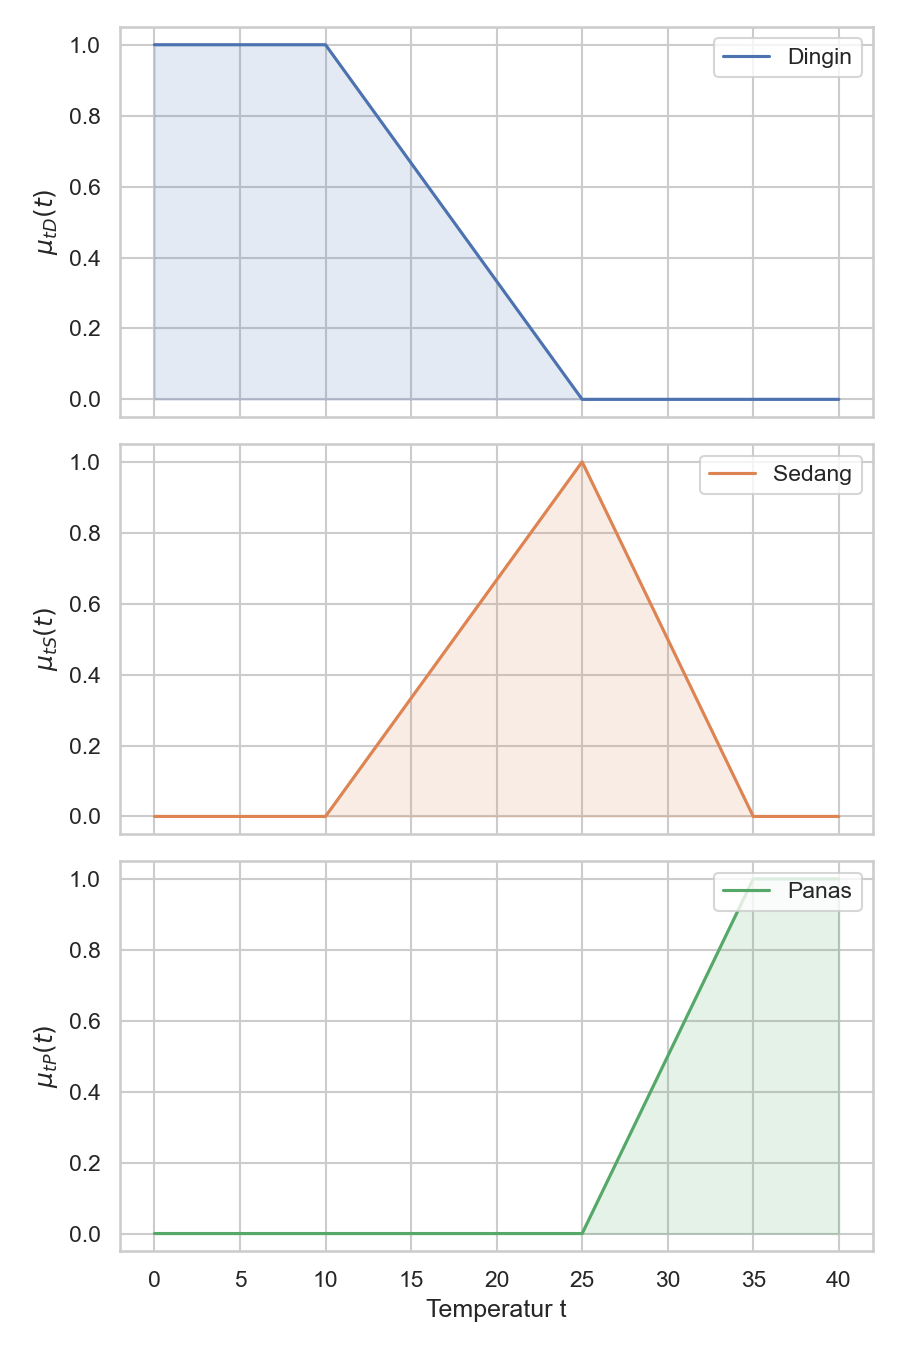
\includegraphics[width=0.75\linewidth]{../plots/memberships.png}
  \caption{Fungsi keanggotaan segitiga untuk tiga himpunan fuzzy temperatur.
    \textit{Atas}: $\mu_{tD}(t)$ -- Dingin (bahu kiri: $\mu=1$ untuk $t \le 10$, turun linear ke 0 pada $t=25$).
    \textit{Tengah}: $\mu_{tS}(t)$ -- Sedang (segitiga penuh, naik dari $t=10$, puncak di $t=25$, turun ke $t=35$).
    \textit{Bawah}: $\mu_{tP}(t)$ -- Panas (bahu kanan: naik dari $t=25$, $\mu=1$ untuk semua $t \ge 35$).}
  \label{fig:memberships}
\end{figure}

Dari Gambar~\ref{fig:memberships} dapat diamati karakteristik setiap himpunan:
\begin{itemize}
  \item \textbf{Dingin} $\mu_{tD}(t)$: derajat keanggotaan bernilai 1 untuk semua
        $t \le 10\,^{\circ}\mathrm{C}$ (bahu kiri), lalu menurun secara linear hingga
        0 pada $t = 25\,^{\circ}\mathrm{C}$.
  \item \textbf{Sedang} $\mu_{tS}(t)$: naik linear dari 0 pada $t=10$ menuju puncak 1 di $t=25$,
        lalu turun linear ke 0 pada $t=35$.
  \item \textbf{Panas} $\mu_{tP}(t)$: naik linear dari 0 pada $t=25$ menuju 1 di
        $t = 35\,^{\circ}\mathrm{C}$, kemudian bernilai 1 untuk semua $t \ge 35\,^{\circ}\mathrm{C}$
        (bahu kanan).
\end{itemize}

\subsection*{Verifikasi Numerik}

Tabel~\ref{tab:verifikasi} merangkum nilai derajat keanggotaan pada $t = 32{,}5\,^{\circ}\mathrm{C}$
untuk tiga kombinasi parameter yang digunakan dalam pengujian unit.

\begin{table}[htbp]
  \centering
  \caption{Nilai derajat keanggotaan pada $t = 32{,}5\,^{\circ}\mathrm{C}$}
  \begin{tabular}{c c c c c}
    \toprule
    $t$ & $a$ & $b$ & $c$ & $\mu(t;\,a,b,c)$ \\
    \midrule
    32.5 &  0 & 10 & 25 & 0.00 \\
    32.5 & 10 & 25 & 35 & 0.25 \\
    32.5 & 25 & 35 & 35 & 0.75 \\
    \bottomrule
  \end{tabular}
  \label{tab:verifikasi}
\end{table}

Perhitungan manual untuk baris kedua dan ketiga:
\begin{equation}
  \mu(32.5;\, 10, 25, 35) = \frac{35 - 32.5}{35 - 25} = \frac{2.5}{10} = 0.25
\end{equation}
\begin{equation}
  \mu(32.5;\, 25, 35, 35) = \frac{32.5 - 25}{35 - 25} = \frac{7.5}{10} = 0.75
\end{equation}

% ===========================================================================
\section*{Pengujian Unit}
% ===========================================================================

Validasi implementasi dilakukan dengan tiga \textit{unit test} pada
\texttt{tests/test\_fuzzy.py} menggunakan \texttt{unittest}:

\begin{lstlisting}[style=python, caption={tests/test\_fuzzy.py -- unit test fungsi keanggotaan}]
class TestFuzzySuhu(unittest.TestCase):

    def test_di_luar_rentang(self):
        """Nilai suhu di luar rentang harus menghasilkan 0."""
        self.assertEqual(fuzzy_suhu(32.5, 0, 10, 25), 0)

    def test_sisi_turun(self):
        """Nilai suhu pada sisi turun segitiga harus menghasilkan nilai benar."""
        self.assertAlmostEqual(fuzzy_suhu(32.5, 10, 25, 35), 0.25)

    def test_sisi_naik(self):
        """Nilai suhu pada sisi naik segitiga harus menghasilkan nilai benar."""
        self.assertAlmostEqual(fuzzy_suhu(32.5, 25, 35, 35), 0.75)
\end{lstlisting}

Ketiga test tersebut mencakup tiga kondisi kritis:
\begin{enumerate}
  \item \textbf{\texttt{test\_di\_luar\_rentang}}: memastikan fungsi mengembalikan 0
        ketika suhu tidak memenuhi kondisi keanggotaan manapun.
  \item \textbf{\texttt{test\_sisi\_turun}}: memvalidasi perhitungan pada sisi turun
        ($b < t \le c$) fungsi segitiga penuh (Sedang).
  \item \textbf{\texttt{test\_sisi\_naik}}: memvalidasi perhitungan pada sisi naik
        ($a \le t \le b$) untuk fungsi bahu kanan (Panas).
\end{enumerate}

Semua test lulus (\texttt{OK}) saat dijalankan dengan
\texttt{python -m pytest tests/} dari direktori root proyek.

% ===========================================================================
\section*{Kesimpulan}
% ===========================================================================

Tugas 2 berhasil mengimplementasikan fungsi keanggotaan segitiga untuk logika fuzzy
menggunakan Python tanpa dependensi library fuzzy eksternal. Poin-poin utama:

\begin{enumerate}
  \item Fungsi \texttt{fuzzy\_suhu} mengimplementasikan Persamaan~\ref{eq:segitiga}
        dengan penanganan kasus degenerate ($a = b$ dan $b = c$) untuk menghindari
        pembagian dengan nol.
  \item Tiga himpunan fuzzy -- \textbf{Dingin}, \textbf{Sedang}, dan \textbf{Panas} --
        berhasil divisualisasikan dengan parameter yang tertera pada
        Tabel~\ref{tab:params}.
  \item Unit test memvalidasi kebenaran hasil numerik, termasuk kondisi di luar
        rentang, sisi naik, dan sisi turun fungsi segitiga.
  \item Struktur proyek menggunakan direktori \texttt{src/} untuk modul,
        \texttt{tests/} untuk pengujian, dan \texttt{plots/} untuk output gambar,
        sehingga sesuai dengan praktik rekayasa perangkat lunak yang baik.
\end{enumerate}

\bibliographystyle{IEEEtran}
\bibliography{references}

\end{document}
